\documentclass[11pt]{article}
\usepackage[automark]{scrpage2}
\usepackage{lastpage}
\usepackage{pdfpages}
\usepackage[top=3.5cm, bottom=2.5cm, left=2.5cm, right=2.5cm]{geometry}

\pagestyle{scrheadings}
\addtolength{\voffset}{-15pt}
\ihead{Mobile Computing/Alarm-App\\ Gruppe 5 Bedienungsanleitung}  
\ohead{Adrian Kurth, Jannes Peters\\ Tjark Kl{\"u}ttermann, Jan Peter Lamp}
\setheadsepline{0.4pt}
\setfootsepline{0.4pt}
\ifoot{Flensburg University of Applied Sciences}  \ofoot{\thepage\space of \pageref{LastPage}}

\begin{document}
	\begin{titlepage}
		\centering
		{\scshape\LARGE Hochschule Flensburg\par}
		\vspace{1cm}
		{\scshape\Large Mobile Computing\par}
		\vspace{1.5cm}
		{\huge\bfseries Alarm-App Bedienungsanleitung\par}
		\vspace{2cm}
		{\Large\itshape Adrian Kurth, Jannes Peters, Tjark Kl{\"u}ttermann und Jan Peter Lamp\par}
		
		
		\vfill
		
		% Bottom of the page
		{\large \today\par}
	\end{titlepage}
\section{Vorbereitung}
Das Smartphone, auf dem die Alarm-App laufen soll, muss mindestens die Android-Version 4.0.3 besitzen und {\"u}ber eine Kamera verf{\"u}gen. Zudem muss die App "OpenCV Manager" installiert sein.
\section{Benutzung}
Um die App benutzen zu k{\"o}nnen, muss diese das Recht haben, die Kamera zu benutzen. Beim ersten Start der App {\"o}ffnet sich ein Fenster, welches nach diesem Recht fragt.\\
Wenn die App ge{\"o}ffnet wird, sieht man auf der linken Seite das Kamerabild. Auf der rechten Seite sieht man von oben nach unten:
\begin{itemize}
	\item Aktueller Status
	\item Kurzer Text, ob der Alarm ausgel{\"o}st wurde
	\item Schalter um den Ton zu aktivieren
	\item Toggle-Button um den Alarm scharf zu stellen ("On/Off")
\end{itemize}
\begin{center}
	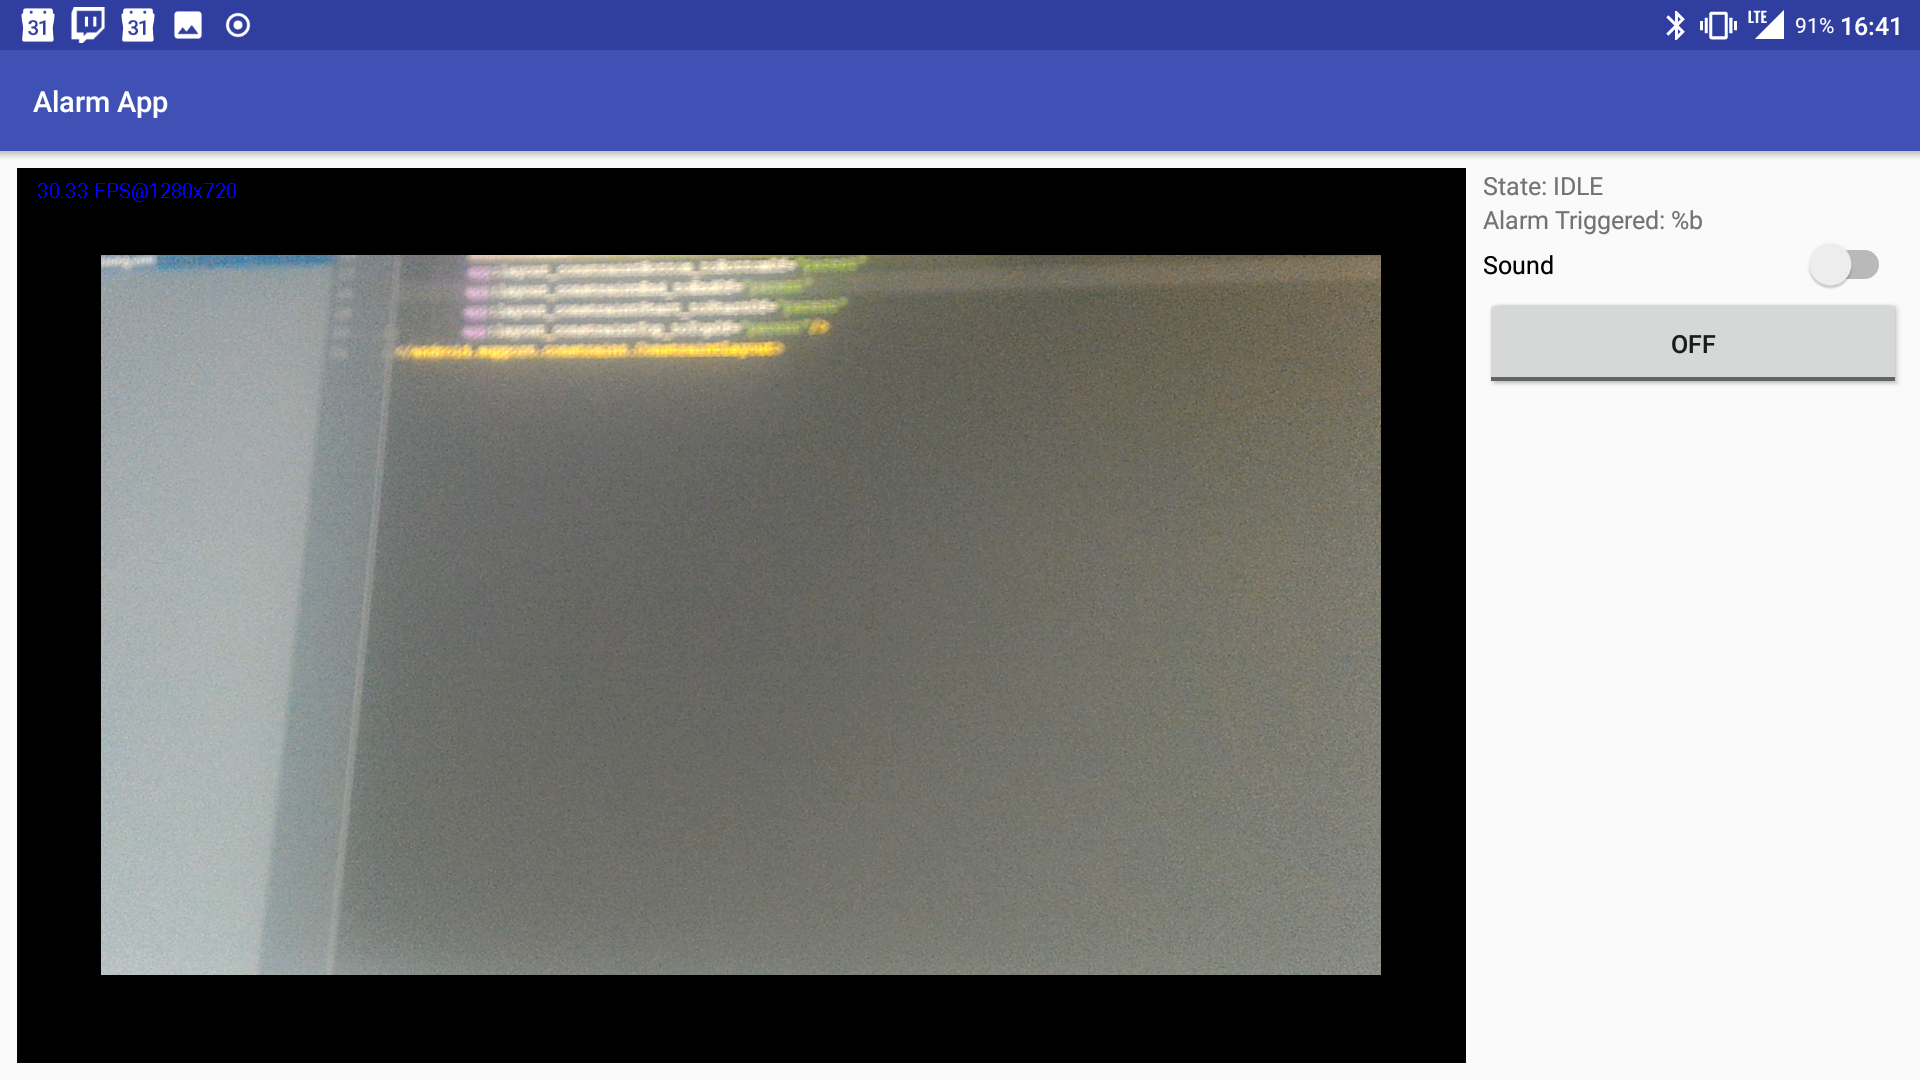
\includegraphics[scale=0.2]{clean-shot.png}
\end{center}
Durch bet{\"a}tigen des Buttons wird die Aktivierung des Alarms eingeleitet. Zun{\"a}chst hat der Benutzer 10 Sekunden Zeit den Raum zu verlassen. Darauf folgen 10 Sekunden Kalibrierungszeit. In dieser Zeit sollte das Smartphone ruhig liegen und nicht bewegt werden. Nach der Kalibrierung ist die App scharf geschaltet. \\
Bei starken Bewegungen oder beim Ein-/Ausschalten des Lichts wird der Alarm ausgel{\"o}st und es wird der Alarmsound abgespielt, soweit dieser eingeschaltet ist. Durch erneutes Bet{\"a}tigen des Toggle-Buttons wird der Alarm ausgestellt.
\end{document}